% Template for Cogsci submission with R Markdown

% Stuff changed from original Markdown PLOS Template
\documentclass[10pt, letterpaper]{article}

\usepackage{cogsci}
\usepackage{pslatex}
\usepackage{float}
\usepackage{caption}

% amsmath package, useful for mathematical formulas
\usepackage{amsmath}

% amssymb package, useful for mathematical symbols
\usepackage{amssymb}

% hyperref package, useful for hyperlinks
\usepackage{hyperref}

% graphicx package, useful for including eps and pdf graphics
% include graphics with the command \includegraphics
\usepackage{graphicx}

% Sweave(-like)
\usepackage{fancyvrb}
\DefineVerbatimEnvironment{Sinput}{Verbatim}{fontshape=sl}
\DefineVerbatimEnvironment{Soutput}{Verbatim}{}
\DefineVerbatimEnvironment{Scode}{Verbatim}{fontshape=sl}
\newenvironment{Schunk}{}{}
\DefineVerbatimEnvironment{Code}{Verbatim}{}
\DefineVerbatimEnvironment{CodeInput}{Verbatim}{fontshape=sl}
\DefineVerbatimEnvironment{CodeOutput}{Verbatim}{}
\newenvironment{CodeChunk}{}{}

% cite package, to clean up citations in the main text. Do not remove.
\usepackage{apacite}

% KM added 1/4/18 to allow control of blind submission


\usepackage{color}

% Use doublespacing - comment out for single spacing
%\usepackage{setspace}
%\doublespacing


% % Text layout
% \topmargin 0.0cm
% \oddsidemargin 0.5cm
% \evensidemargin 0.5cm
% \textwidth 16cm
% \textheight 21cm

\title{Information is Not Communicated Uniformly: Evidence from Spoken and
Written Corpora}


\author{Josef Klafka \and Daniel Yurovsky \\
        \texttt{\{jklafka, yurovsky\}@uchicago.edu} \\
       Department of Psychology \\ University of Chicago}

\begin{document}

\maketitle

\begin{abstract}
We provide evidence against the popular Uniform Information Density
hypothesis (Levy \& Jaeger, 2007) which proposes that information is
transmitted at a constant rate close to channel capacity in human
communication. Using a method based on the original Genzel \& Charniak
(2002) entropy measure, we construct a word-level model for entropy
applicable to both spoken and written corpora. We apply this model to
corpora from Wikipedia in well over a hundred languages. We find that
the Uniform Information Density hypothesis does not predict the outcome
of our word-level entropy model, but also that the by-word entropy
distribution of a language is related to the typological features of the
language. We use this evidence to suggest that people do not communicate
information at a uniform rate, but that information distribution varies
from language to language based on phonogical, morphological and
syntactic features.

\textbf{Keywords:}
Entropy; information; information theory; communication
\end{abstract}

\section{Introduction}\label{introduction}

Over 7,000 languages are spoken around the modern world (Simons \&
Fenning, 2018). These language vary along many dimensions, but all share
a core goal: communicating information. If speakers and writers of these
languages act near-optimally to achieve their communicative goals,
regularities of use across these diverse languages can be explained by a
rational theory of communication (Anderson, 1991). Information theory, a
mathematical framework developed by Shannon (1948) to describe the
transmission and decoding of signals, has been a unifying language for
the recent development of such theories in human and machine language
processing (Jelinek, 1976; R. P. Levy \& Jaeger, 2007).

These theories model the process of communication as transmission of
information over a noisy channel. The producer begins with an intended
meaning, packages this meaning into a linguistic format, and then sends
it to the receiver over a communcative channel. The receiver must then
decode from the signal they receive on their end of the chanel the
producer's intended meaning. The problem is that the channel is noisy,
and sometimes the signal can get corrupted (e.g.~the producer can
misspeak, or the receiver can mishear). In order to maximize the
probability that the correct meaning is transmitted, these theories
predict that producers should choose linguistic messages that keep the
rate of information across words constant. The intuition is that if the
receiver misperceives a word, and that word contains most of the
information in the sentence, then the communication will have failed.
Because producers cannot predict which word a speaker will mishear,
their best strategy is spread the information evenly across all of the
words in a sentence, i.e.~maintain \emph{uniform information density}
(Genzel \& Charniak, 2002; R. P. Levy \& Jaeger, 2007).

The original evidence in R. P. Levy \& Jaeger (2007) finds that the
insertion of complementizers in relative clauses in English corresponds
to where neighboring words have high information content. Similarly,
Frank \& Jaeger (2008) argues that contradictions in English such as
``you're'' do not occur when neighboring words are highly informative.
The evidence in favor of UID largely been situation-specific and
English-language driven, while the hypothesis itself has been applied
broadly over the past decade. Applications include determining whether
linguistic alignment takes place (Jaeger \& Snider, 2013), Zipfian word
length distributions (Piantadosi, Tily, \& Gibson, 2011), communication
efficiency (Mahowald, Fedorenko, Piantadosi, \& Gibson, 2013), dialogue
and turn-taking (Xu \& Reitter, 2018) and the significance of ambiguity
in language (Piantadosi, Tily, \& Gibson, 2012), among other research.

However, other recent work has contradicted the UID hypothesis. Similar
to the original R. P. Levy \& Jaeger (2007), Zhan \& Levy (2018) focuses
on information distribution at particular points in sentences. Zhan \&
Levy (2018) finds that more information-rich classifiers in Mandarin
Chinese are produced when production of the neighboring noun is
difficult, not when the information content is high. On a sentential
level, Jain, Singh, Ranjan, Rajkumar, \& Agarwal (2018) examine word
order across spoken sentences in Hindi, a freer word order language than
English, and find that information density has no significant effect on
word order.

Recently, Yu, Cong, Liang, \& Liu (2016) developed a more direct test of
the Uniform Information Density hypothesis, applying the logic used by
Genzel \& Charniak (2002) to look at the distribution of information
\emph{within} individual sentences. Because people process language
incrementally--using the previous words in a sentence to predict the
words that will come next, the amount of information that a word
contains when seen in isolation should increase over the course of a
sentence. Analyzing a large corpus of written English, they find a
different pattern: Entropy increases over the first few words of an
utterance and then remains constant until the final word where it again
jumps up (see Figure \ref{fig:our_replication}). Yu et al. (2016)
conclude that the Uniform Information Density hypothesis must not hold
for medial words in a sentence.

We extend and generalize Yu et al. (2016) in three ways: we confirm that
this same pattern is found in spoken English--in both adult and child
speakers. We then examine entropy curves cross-linguistically, finding a
diversity of shapes across the world's languages. Finally, we show that
entropy curves are predictable from the structure of individual
languages, namely word order. Taken together, our results suggest a
refinement of the Uniform Information Density hypothesis: Speakers may
choose to order words in order to preserve uniform information, but they
must do so under prior constraints on word order imposed by the language
they speak.

The UID hypothesis predicts that information transmission rate will tend
towards uniformity in both speech and text. We begin by examining speech
to determine if we obtain the entropy curve shape we expect for spoken
communication. We begin with the same source as R. P. Levy \& Jaeger
(2007) and Jaeger (2010), the Switchboard corpus of adult telephone
conversations. We also examine child-adult conversations in the CHILDES
TalkBank (Brown, 1973; MacWhinney, 2014) corpora database of spoken
adult-child conversations in multiple languages. Children are not fully
developed speakers, so we want to compare the entropy curve we obtain by
computing over the utterances in the CHILDES corpora to the utterances
in the adult-adult Switchboard corpus.

\subsection{Methods}\label{methods}

Yu et al. (2016) challenges the UID hypothesis through examining an
entropy measure across sentence positions within the text portion of the
English-language British National Corpus (BNC) Clear (1993). They
partition the corpus by sentence length in number of words. For each
word position \(X\) of sentences of length \(k\), they define \(w\) as a
unique word occurring in position \(X\). They define \(p(w)\) as the
number of times word \(w\) occurs in position \(X\) divided by the
number of total words that occur in position \(X\) i.e.~the number of
sentences of length \(k\). Then \(p(w)\) is the probability of obtaining
word \(w\) by choosing a word at random in position \(X\) in sentences
of length \(k\).

\[H(X) = \sum\limits_w p(w)\log\big(p(w)\big)\] With this measure, Yu et
al. (2016) compute the unigram entropy at each position of sentences of
each length within the corpus. The result of this method can be plotted
for each utterance length as an \emph{entropy curve}, which can be
visually compared across utterance length to observe the how the unigram
entropy changes across absolute positions in each of the utterances.
Genzel \& Charniak (2002) similarly examine a unigram entropy measure on
sentences, and found that entropy at the sentence level increases
linearly with sentence index within a corpus. UID applies this
uniformity of entropy rate in sentences to all levels of speech, and so
the Yu et al. (2016), which examines text at the word level, should find
an affine function at the word level.

Switchboard {[}To be put in{]}

We used the Providence English corpds from CHILDES. The Providence
corpus recorded interactions between children between 1 and 3 years old
and their parents in the home. We divided the corpus by speaker into
child and non-child categories. We further divided the corpus by
utterance length, so that all sentences of length \(k\) (e.g. \(6\))
were grouped together. Finally, within each utterance length, we
computed the unigram entropy measure for each position.

The entropy curves capture individual variation across positions in
utterances of the same length. This allows us to directly observe and
judge the amount of variation in words that appear in an individual
position of a sentence. For speech data, which for the corpora in the
CHILDES database consists of short and often disconnected utterances
across hours of recordings, the unigram entropy measure is unaffected by
context or lack thereof in utterances by the adults and children in the
corpora. We can directly compare any two positions within utterances to
determine the amount of uncertainty, and therefore information, on
average contained by words within that position of utterances. We are
applying the same approach as in Genzel \& Charniak (2002), but within
sentences instead of across sentences.

\begin{CodeChunk}
\begin{figure*}[h]

{\centering 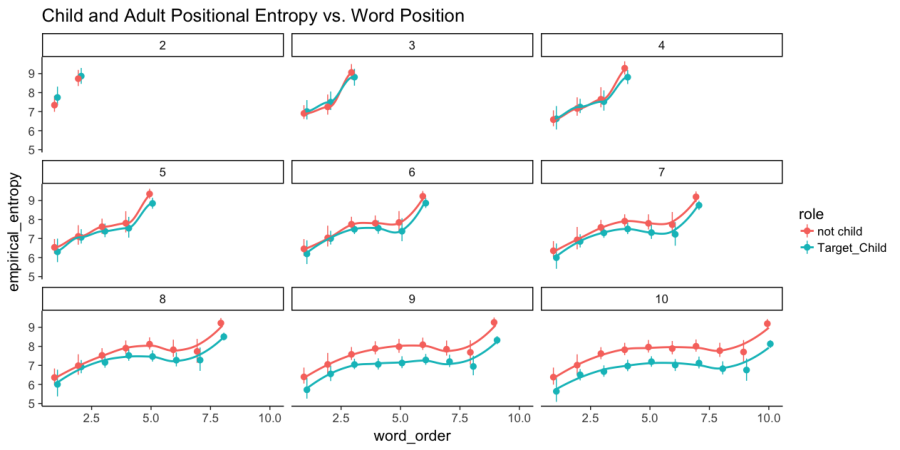
\includegraphics{figs/providence_PE-1} 

}

\caption[Providence corpus unigram entropy]{Providence corpus unigram entropy}\label{fig:providence_PE}
\end{figure*}
\end{CodeChunk}

We also ran this analysis on Spanish and Mandarin corpora from CHILDES.
We used the Shiro corpus for Spanish (Shiro, 2000), which contains
prompted narratives individually collected from over a hundred
Venezualan schoolchildren, half from high SES backgrounds and half from
low SES backgrounds. We used the Zhou dinner corpus for Mandarin Chinese
(Li \& Zhou, 2015), which contains dinner conversations between 5 to
6-year-old children and their parents collected in Shanghai.

For each corpus, we accessed transcripts of the corpus provided through
the TalkBank system and computed over Roman alphabet transcriptions or
transliterations of the original transcriptions. For Mandarin, we used
pinyin transliterations of the utterances in the corpus with demarcated
word boundaries, and for Japanese we used romanji (Roman alphabet)
transliterations of words in the corpus. The Chinese characters used for
writing Mandarin do not normally demarcate word boundaries by spacing
words apart, and for normal Chinese writing including spaces between
word boundaries can have a negative effect on reading times (Bai et al,
2008).

\begin{CodeChunk}
\begin{figure*}[h]

{\centering 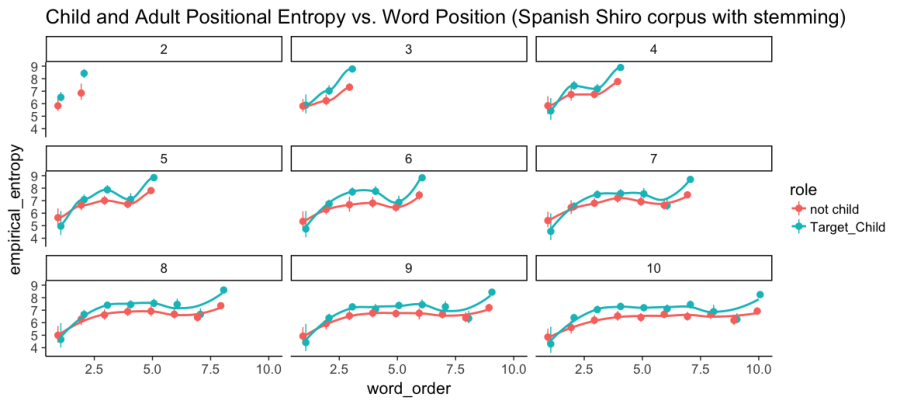
\includegraphics{figs/shiro_PE-1} 

}

\caption[Shiro corpus entropy]{Shiro corpus entropy}\label{fig:shiro_PE}
\end{figure*}
\end{CodeChunk}

\begin{CodeChunk}
\begin{figure*}[h]

{\centering 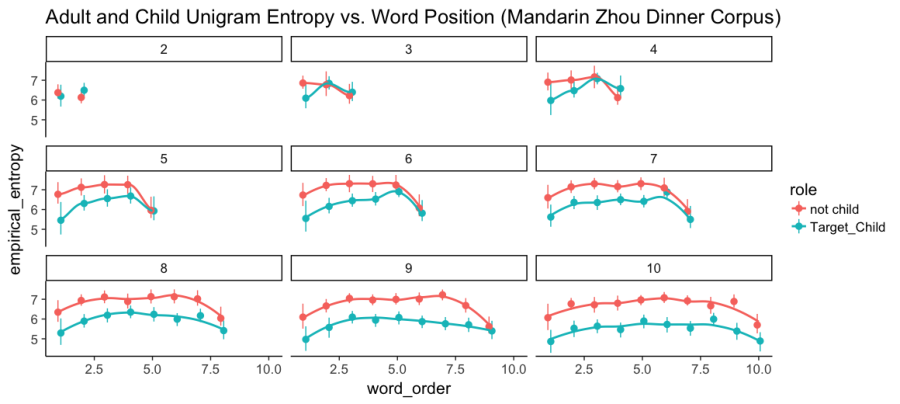
\includegraphics{figs/zhou_PE-1} 

}

\caption[Zhou Dinner corpus entropy]{Zhou Dinner corpus entropy}\label{fig:zhou_PE}
\end{figure*}
\end{CodeChunk}

\subsection{Results \& Analysis}\label{results-analysis}

The adult and child entropy curves track one another almost identically.
This is surprising because UID would predict that the young children in
the corpora who are not fully developed speakers would have more noise
in their distribution of information rates. This not only indicates a
robustness in the unigram entropy curve across speakers, but also across
ages and addressees. We also observed a robustness across corpora for
the same languages, and a robustness across utterance lengths within the
same corpus's entropy curve. This shows that the concept of an ``entropy
curve'' for a specific language is well-founded when considering speech
data.

We found a distinct three-step distribution for English and Spanish
CHILDES corpora, with a slight dip in the penultimate position of each
sentence. The final position of utterances in child-directed speech is
known to be important, dating back to Aslin (1993). The Mandarin corpus
entropy curve, by comparison, has a noticeably lower positional entropy
values in utterance-final positions than in utterance-penultimate
positions.

We attribute the penultimate dip in the English and Spanish entropy
curves to the fact that most of the utterances in the CHILDES English
and Spanish corpora we examined had a determiner such as ``the'' or
``a'' in the second-to-last position of utterances. The beginnings of
utterances in the English and Spanish CHILDES data were usually pronouns
or grammatical subjects, while the final words were grammatical objects
and had a great deal of variation in the exact word that appeared in the
utterance-final position.

These entropy curves are not what would be expected from UID. The
robustness of the three-step distribution for English and its
replication in Spanish do not resemble the affine function we would
expect from UID. The Mandarin entropy curve, which does not at all
resemble either the English/Spanish distribution or the predictions of
UID, suggests that the entropy curve can vary from language to language.
UID predicts that each language should have a similar distribution.

\section{Written data}\label{written-data}

The UID hypothesis also applies to written communication: we expect
people to communicate information at a uniform rate through writing as
well. We use Wikipedia as a source for written data, which provides two
advantages. One, the quantity of data in Wikipedia is large for each
language and two, there are hundreds of languages with Wikipedias. This
allows us to perform the entropy analysis on a much greater scale and to
directly compare the results of the entropy analysis on each language to
one another, and ultimately to predict what typological features of a
language help determine its entropy curve, if any. We will describe our
method of harvesting and distilling text data from each Wikipedia as
well as how we compare the entropy curves from each language to one
another.

\subsection{Methods}\label{methods-1}

Using Giuseppe Attardi's Wikiextractor tool
\footnote{https://github.com/attardi/wikiextractor}, we extracted the
text corpora for \(165\) languages from Wikipedia by downloading a
stored collection of Wikipedia entries in each langauge and randomly
selecting several thousand articles from each Wikipedia language. Each
language corpus was cleaned and limited to sentences between \(6\) and
\(50\) words. Similar to our process for the Switchboard and CHILDES
spoken corpora, we divided each corpus by sentence length, and then
computed the unigram entropy measure on each word position within each
sentence length. We wanted to directly compare and classify the unigram
entropy curves of the languages from Wikipedia. We computed three slope
treatments of each curve. In the \emph{absolute} treatment, with
sentence length denoted as \(n\), we computed the slope between
positions \(1\) and \(2\), positions \(2\) and \(3\), positions \(3\)
and \(n-2\), positions \(n-2\) and \(n-1\) and positions \(n-1\) and
\(n\). For the short utterances appearing the CHILDES speech corpora we
examined, these appeared to be important junctions in the distributions,
with a seeming plateau in the middle of the unigram entropy curve for
each of the language corpora we examined in CHILDES.

However, because the portion of sentences of length greater than \(10\)
in the Wikipedia corpora were significantly larger than the CHILDES
corpora, then we also computed relative slope treatments. In the
\emph{relative 5} treatment, we computed the slopes between \(0\%\) and
\(20\%\), \(20\%\) and \(40\%\), \(40\%\) and \(60\%\), \(60\%\) and
\(80\%\) and \(80\%\) and \(100\%\) of the relative word positions in
each sentence. When one of these percentages was not a whole number,
then the closest whole number position was used instead for slope
calculation. In the \emph{relative 10} treatment, we computed the slopes
between every \(10\%\) of the relative word positions in each sentence.
Each comparative slope within each treatment was averaged together
between different sentence lengths, for example in the \emph{relative 5}
treatment then all of the \(0\%\) to \(20\%\) slopes were averaged
together. This created three treatments for the entropy curve for each
langauge in the Wikipedia database.

{[}Put in an illustration of the slope sections and treatments here?{]}

\subsection{Results and Analysis}\label{results-and-analysis}

In the \emph{absolute} and \emph{relative 5} treatments, each language
is embedded in \(5\)-dimensional space. In the \emph{relative 10}
treatment, each language is embedded in \(10\)-dimensional space. This
allows for direct comparison between languages on Wikipedia using cosine
similarity and moreover for unsupervised clustering analysis to compare
the results of the Wikipedia entropy analysis to known typological
features within the langauges in the Wikipedia dataset. To determine
which phonological, morphological and syntactic features affected the
embedding of a language in the Wikipedia dataset, we looked at the list
of \(144\) linguistic features in World Atlas of Language Structures
(Dryer \& Haspelmath, 2013). We limited the languages in the WALS
database to only those in our Wikipedia dataset and performed
missing-value imputation to obtain the features not coded in WALS for
the languages from Wikipedia.

One approach is to cluster the languages used in the Wikipedia analysis
on the basis of WALS features and then directly compare the WALS
clustering results with the results of the hierarchical clustering on
the Wikipedia slope data for each of the different treatments using
clustering similarity evaluation methods such as the Rand index (Rand,
1971). However, the problem then arises of which combination of WALS
features and how many features to include in the clustering analysis.
This is a computationally intractable operation. Additionallly, deciding
how many clusters to use in an unsupervised clustering analysis is an
unsolved problem in machine learning.

We instead check the effects of individual features on the embeddings of
languages in the different treatments. We computed pairwise cosine
similarity between each pair of language vectors within a treatment. For
a subset of WALS features which had values entered for most of the
languages we obtained from Wikipedia, we used a generalized linear model
to see whether the cosine similarity between languages mattered in
predicting if the languages shared the same value for a WALS feature.
For eight features and \(45\) languages, we found this to be true. The
table below shows the results for the generalized linear model we
computed using WALS features and the absolute treatment.

\begin{table}[tb]
\centering
\begin{tabular}{llrrrr}
  \hline
feature & term & estimate & std.error & statistic & p.value \\ 
  \hline
83A & cosine & 1.84 & 0.01 & 178.22 & 0.00 \\ 
  95A & cosine & 1.90 & 0.01 & 170.98 & 0.00 \\ 
  81A & cosine & 1.51 & 0.01 & 153.70 & 0.00 \\ 
  97A & cosine & 1.58 & 0.01 & 136.81 & 0.00 \\ 
  144A & cosine & 0.88 & 0.01 & 74.43 & 0.00 \\ 
  138A & cosine & 0.40 & 0.01 & 46.12 & 0.00 \\ 
  87A & cosine & 0.33 & 0.01 & 39.91 & 0.00 \\ 
  143A & cosine & 0.37 & 0.01 & 39.74 & 0.00 \\ 
  82A & cosine & 0.03 & 0.01 & 3.23 & 0.00 \\ 
   \hline
\end{tabular}
\end{table}

Cosine distance played some role in the feature determination. The top
features were \(83\), \(81\), \(95\) and \(97\), which all characterize
word order. This makes intuitive sense, and indicates that for this
small subset of features and subset of languages that the embeddings in
the slope space are related to the WALS features. Therefore typological
features play a role in determining the positional entropy values for a
language. This means that the entropy curves are in some way structured
by the syntactic, morphological and phonological features of a language.

\section{Conclusions}\label{conclusions}

In this paper, we have characterized and applied a model based on Genzel
\& Charniak (2002) for distinguishing entropy at each word position
within sentences. In doing so, we have provided evidence against the
Uniform Information Density hypothesis. Our work indicates that
information is not distributed uniformly throughout an utterance
regardless of languages, but that languages possess a characteristic
information distribution determined by their syntactic, morphological
and phonological features.

Our work has focused on words within sentences in both speech and text
across typologically diverse languages. Other researchers have explored
information rate cross-linguistically as a single number characterizing
each language, most notably including Aylett \& Turk (2004). That work
characterizes information rate as information per unit time, and is
complementary to the work we accomplish here. Languages may possess both
an overall information transfer rate, showing the average amount of
semantic information transmitted per syllable or word, and an entropy
distribution indicative of the language's information distribution.

Research has indicated the effects of surprisal on fixation duration
during eye-tracking studies (Demberg \& Keller, 2008) (Boston et al.,
2008) (Smith \& Levy, 2013). Higher surprisal of a word is on average
predictive of higher fixation duration. The \emph{wrap-up effect} states
that when a person reads written text, he or she will process
sentence-final words more slowly on average then sentence-medial or
sentence-initial words, due to integrating information from the entire
sentence to form a final understanding of the sentence's meaning (Stowe
et al., 2018) (Kuperman et al., 2010). The wrap-up effect is drawn from
evidence in English, German and Dutch, all of which are languages with a
large final increase in their entropy curve from our study. We aim to
see in the future if as a consequence of our work in this paper, the
wrap-up effect falls out from the final jump in the entropy curves in
some languages. We would analyze eye-tracking data from languages with
low positional entropy in sentence-final positions. Since the lexical
surprisal metric in eye-tracking and our positional entropy metric are
both measures of log-probability surprisal, then in languages such as
Hindi where the sentence-final positional entropy values are low we
expect to find no wrap-up effect.

\section{Acknowledgements}\label{acknowledgements}

{[}Not here yet.{]}

\section{References}\label{references}

\setlength{\parindent}{-0.1in} \setlength{\leftskip}{0.125in} \noindent

\hypertarget{refs}{}
\hypertarget{ref-anderson1991}{}
Anderson, J. R. (1991). The adaptive nature of human categorization.
\emph{Psychological Review}, \emph{98}(3), 409.

\hypertarget{ref-brown1973}{}
Brown, R. (1973). \emph{A first language: The early stages.} Harvard U.
Press.

\hypertarget{ref-clear1993british}{}
Clear, J. H. (1993). The british national corpus. \emph{The Digital
World}, 163--187.

\hypertarget{ref-frank2008speaking}{}
Frank, A. F., \& Jaeger, T. F. (2008). Speaking rationally: Uniform
information density as an optimal strategy for language production. In
\emph{Proceedings of the annual meeting of the cognitive science
society} (Vol. 30).

\hypertarget{ref-genzel2002}{}
Genzel, D., \& Charniak, E. (2002). Entropy rate constancy in text. In
\emph{Proceedings of the 40th annual meeting on association for
computational linguistics} (pp. 199--206). Association for Computational
Linguistics.

\hypertarget{ref-jaeger2010}{}
Jaeger, T. F. (2010). Redundancy and reduction: Speakers manage
syntactic information density. \emph{Cognitive Psychology},
\emph{61}(1), 23--62.

\hypertarget{ref-jaeger2013}{}
Jaeger, T. F., \& Snider, N. E. (2013). Alignment as a consequence of
expectation adaptation: Syntactic priming is affected by the prime's
prediction error given both prior and recent experience.
\emph{Cognition}, \emph{127}(1), 57--83.

\hypertarget{ref-jain2018}{}
Jain, A., Singh, V., Ranjan, S., Rajkumar, R., \& Agarwal, S. (2018).
Uniform information density effects on syntactic choice in hindi. In
\emph{Proceedings of the workshop on linguistic complexity and natural
language processing} (pp. 38--48).

\hypertarget{ref-jelinek1976}{}
Jelinek, F. (1976). Continuous speech recognition by statistical
methods. \emph{Proceedings of the IEEE}, \emph{64}(4), 532--556.

\hypertarget{ref-levy2007}{}
Levy, R. P., \& Jaeger, T. F. (2007). Speakers optimize information
density through syntactic reduction. In \emph{Advances in neural
information processing systems} (pp. 849--856).

\hypertarget{ref-macwhinney2014}{}
MacWhinney, B. (2014). \emph{The childes project: Tools for analyzing
talk, volume ii: The database}. Psychology Press.

\hypertarget{ref-mahowald2013}{}
Mahowald, K., Fedorenko, E., Piantadosi, S. T., \& Gibson, E. (2013).
Info/information theory: Speakers choose shorter words in predictive
contexts. \emph{Cognition}, \emph{126}(2), 313--318.

\hypertarget{ref-piantadosi2011}{}
Piantadosi, S. T., Tily, H., \& Gibson, E. (2011). Word lengths are
optimized for efficient communication. \emph{Proceedings of the National
Academy of Sciences}, \emph{108}(9), 3526--3529.

\hypertarget{ref-piantadosi2012}{}
Piantadosi, S. T., Tily, H., \& Gibson, E. (2012). The communicative
function of ambiguity in language. \emph{Cognition}, \emph{122}(3),
280--291.

\hypertarget{ref-shannon1948}{}
Shannon, C. E. (1948). A mathematical theory of communication.
\emph{Bell System Technical Journal}, \emph{27}(3), 379--423.

\hypertarget{ref-simons2018}{}
Simons, G. F., \& Fenning, C. D. (Eds.). (2018). \emph{Ethnologue:
Languages of the world, 21st edition}. Dallas, Texas: SIL International.

\hypertarget{ref-xu2018}{}
Xu, Y., \& Reitter, D. (2018). Information density converges in
dialogue: Towards an information-theoretic model. \emph{Cognition},
\emph{170}, 147--163.

\hypertarget{ref-yu2016}{}
Yu, S., Cong, J., Liang, J., \& Liu, H. (2016). The distribution of
information content in english sentences. \emph{arXiv Preprint
arXiv:1609.07681}.

\hypertarget{ref-zhan2018}{}
Zhan, M., \& Levy, R. (2018). Comparing theories of speaker choice using
a model of classifier production in mandarin chinese. In
\emph{Proceedings of the 2018 conference of the north american chapter
of the association for computational linguistics: Human language
technologies, volume 1 (long papers)} (Vol. 1, pp. 1997--2005).

\bibliographystyle{apacite}


\end{document}
